
\section{Software-Entwurf}

Ziele de Entwurfsphase:
\begin{itemize}
    \item Entwerfen einer Software-\textbf{Architektur}
    \item Spezifikation des Funktions- und Leistungsumfangs der \textbf{Systemkomponenten}
    \item Detaillierung der Systemkomponenten durch Beschreibung ihrer Operationen
\end{itemize}

\subsection{Software-Grobentwurf}

\subsubsection{Software-Architektur}
Eine \textbf{Software-Architektur} beschreibt die Struktur des Software-Systems durch die Systemkomponenten und ihre Beziehungen untereinander.\\
eine \textbf{Systemkomponente} ist ein abgegrenzter Teil eines Software-Systems.
Sie dient als Baustein f"ur die physikalische und logische Struktur einer Anwendung.
Beispiel f"ur Systemkomponenten sind Funktionen/Prozeduren, abstrakte Datentypen, Klassen.

\subsubsection{Ziel des Sotfware-Grobentwurfs}
Ziel des \textbf{Software-Grobentwurfs} ist es, f"ur das zu entwerfende Produkt eine Software-\textbf{Architektur} zu erstellen, die die funktionalen und nicht-funktionalen \textbf{Produktanforderungen} sowie allgemeine und produktspezifische \textbf{Qualit"atsanforderungen} erf"ullt und die \textbf{Schnittstellen} zur Umgebung versorgt.

\subsubsection{Einzusetzende Prinzipien}
Prinzip der \textbf{Zerlegung}\\
$\Rightarrow$ Aufteilung des Systems in miteinander interagierende Bausteine\\
Prinzip der \textbf{Abstraktion}\\
$\Rightarrow$ Identifikation eines Teilsystems mit der funktionalen Rolle, die es im Gesamtsystem zu "ubernehmen hat, zun"achst ohne Ber"ucksichtigung seiner Implementierungsdetails

\subsubsection{Top-Down- und Bottom-Up-Entwurf}
\begin{itemize}
    \item \textbf{Top-Down}-Vorgehensweise
    \begin{itemize}
        \item Spezialisierung
        \item schrittweise Verfeinerung
        \item das Gesamtsystem wird schrittweise in Teilsysteme zerlegt
    \end{itemize}
    \item \textbf{Bottom-Up}-Vorgehensweise
    \begin{itemize}
        \item Generalisierung
        \item schrittweise Verallgemeinerung
        \item das Gesamtsystem wird schrittweise aus Teilsystemen zusammengesetzt
    \end{itemize}
\end{itemize}

Beise Vorgehensweisen sind kombinierbar.


\subsection{Klassische Architekturmodelle}

\subsubsection{Architekturmodelle}
\begin{itemize}
    \item \textbf{Blockdiagramm}\\
    $\Rightarrow$ sehr allg. Darstellung, geeignet als allererster Ansatz
    \item \textbf{Datenspeichermodell}\\
    $\Rightarrow$ geeignet speziell f"ur den Einsatz globaler Datenbanken
    \item \textbf{Schichtenmodell}\\
    $\Rightarrow$ hierarchische Anordnung zunehmend abstrahierter Sichten
    \item \textbf{Client/Server-Modell}\\
    $\Rightarrow$ gemeinsamer Zugriff auf verteilte Dienste
    \item \textbf{Verteiltes System}\\
    $\Rightarrow$ Verteilung des Softwaresystems "uber mehrere Rechner
\end{itemize}

\subsubsection{Objektkommunikation "uber ein ORB}
\#\#\# \textbf{TODO} \#\#\#



\subsection{Koh"asion und Kopplung}

\subsubsection{Kopplung}
F"ur die Qualit"at einer Architektur spielt vor allem der \textbf{Grad der Interaktion} zwischen den Komponenten eine wichtige Rolle.\\
Der Grad der Interaktion zwischen zwei Komponenten wird als \textbf{Kopplung} der beiden Komponenten bezeichnet.\\
Die Modularisierung gewinnt an \textbf{Transparenz} und \textbf{Wartbarkeit}, wenn zwischen den Komponenten nur wenige und einfache Abh"angigkeiten existieren.\\
Ziel des Grob-Entwurfs muss deshalb eine m"oglichst \textbf{geringe Kopplung} sein.\\

\subsubsection{Koh"asion}
Im allgemeinen erzielt man eine niedrige Kopplung, wenn man stark \textbf{zusammenh"angende (Teil-)Funktionalit"aten} in einer gemeinsamen Komponente unterbringt.\\
Der Grad der funktionalen bindung innerhalb einer Komponente wird als \textbf{Koh"asion} bezeichnet.\\
Die Modulariesierung gewinnt an \textbf{Transparenz} und \textbf{Wartbarkeit}, wenn jede Komponente nur aus stark funktional zusammenh"angenden Teilen besteht.\\
Ziel des Grob-Entwurfs muss deshalb eine m"oglichst \textbf{hohe Koh"asion} sein.\\

\subsubsection{Kopplungsarten}
{\color[HTML]{008000}{5.Data coupling}}\\
{\color[HTML]{9ACD32}{4. Stamp coupling}}\\
{\color[HTML]{FFD700}{3. Control coupling}}\\
{\color[HTML]{FFA500}{2. Common coupling}}\\
{\color[HTML]{FF0000}{1. Content coupling}}\\

\subsubsection{Content Coupling}
Zwei Module $p$ und $q$ sind \textbf{inhaltsgekoppelt}, wenn ein Modul $p$ unmittelbare Auswirkungen auf den Inhalt bzw. auf den auszuf"uhrenden Codeteil eines anderen Moduls $q$ haben kann.
Dabei beruht die Inhaltskopplung \textbf{nicht} auf einem \textbf{eigentlichen Aufruf} von $q$ durch $p$; vielmehr wird die Ausf"uhrung von evtl. modifizierten codteilen von $q$ durch $p$ direkt initiiert.

\subsubsection{Common Coupling}
Zwei Module sind \textbf{datenextern} (\textbf{global}, \textbf{"uber globale Daten}) gekoppelt, falls beide auf gemeinsame globale Daten schreibend/lesend zugreifen k"onnen.

\subsubsection{Control Coupling}
Zwei Module besitzen \textbf{Kontrollkopplung}, wenn ein $p$ ein kontrollflussbestimmendes Element an Modul $q$ "ubermittelt.

\subsubsection{Stamp Coupling}
Zwei Module besiten \textbf{Datenstrukturkopplung}, falls eine Datenstruktur als Parameter "ubergeben wird, das aufgerufene Modul aber \textbf{nur Teile der Datenstruktur} verwendet.

\subsubsection{Data Coupling}
Zwei Module sind \textbf{datengekoppelt}, wenn sie Informationen "uber Parameter austauschen die homogene Daten sind:
\begin{itemize}
    \item einfache Daten
    \item Datenstrukturen, deren Elemente alle vom aufgerufenen Modul verwendet werden
\end{itemize}


\subsubsection{Koh"asionsarten}

\begin{enumerate}
    \item Informational cohesion
    \item Functional cohesion
    \item Sequential cohesion
    \item Communicational cohesion
    \item Procedural cohesion
    \item Temporal cohesion
    \item Logical cohesion
    \item Coincidental cohesion
\end{enumerate}

\subsubsection{Coincidental Cohesion}
Ein Modul hat \textbf{zuf"allige Koh"asion} wenn es mehrere, vollkommen unzusammeng"angende Aktionen durchf"uhrt.

\subsubsection{Logical Cohesion}
Ein Modul hat \textbf{logische Koh"asion}, wenn es eine menge verwandter (zum Teil alternativer) Funktionalit"aten anbietet.

\subsubsection{Temporal Cohesion}
Ein Modul hat \textbf{zeitliche Koh"asion} wenn es eine Reihe von Aktionen in zeitlichem Zusammenhang ausf"uhrt.\\
Die \textbf{Reihenfolge} ist dabei \textbf{irrelevant}.

\subsubsection{Procedural Cohesion}
Ein Modul hat \textbf{prozeduale Koh"asion}, wenn es eine Reihe von Aktionen auf unterschiedlichen Daten in zeitlihcer Abfolge durchf"uhrt.\\
Die \textbf{Reihenfolge} ist dabei \textbf{relevant}.

\subsubsection{Communicative Cohesion}
Ein Modul hat \textbf{kommunikative Bindung}, wenn es eine Reihe von Aktionen auf \textbf{gemeinsame} Daten auf"uhrt.\\
Die Reihenfolge ist dabei irrelevant.

\subsubsection{Sequential Cohesion}
Ein Modul hat \textbf{sequentielle} Koh"asion, wenn es eine Reihe von AKtionen in sequentieller Abfolge auf"uhrt.\\
Ausgabedaten werden als Eingabedaten weiterverarbeitet.

\subsubsection{Functional Cohesion}
Ein Modul hat \textbf{funktionale Koh"asion}, wenn alle seine Elemente zur Ausf"uhrung einer und nur einer Aufgabe beitragen.

\subsubsection{Informational Cohesion}
Ein Modul hat \textbf{Informationskoh"asion}, wenn es eine Reihe von Operationen, jede mit eigenem Eingang/Ausgang und \textbf{unabh"angigem} Code, auf der selben Datenstruktur druchf"uhren kann.

\subsubsection{Zusammenfassung von Koh"asionsgraden}

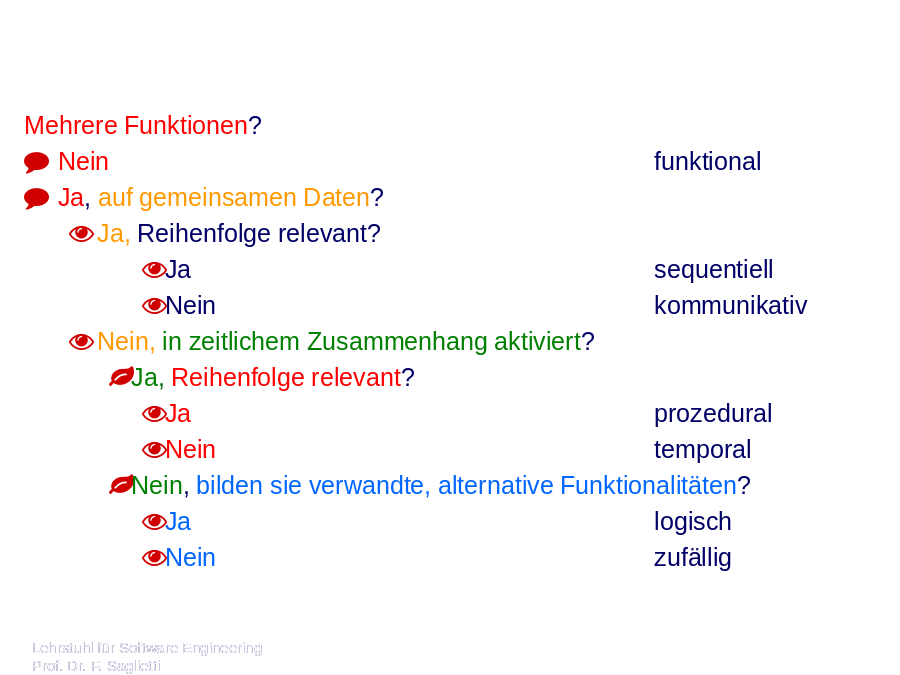
\includegraphics[scale=0.5]{inc/Softwareentwurf/ZusammenfassungKohaesionsgrade.png}

\subsubsection{Zusammenfassung: Koh"asion}

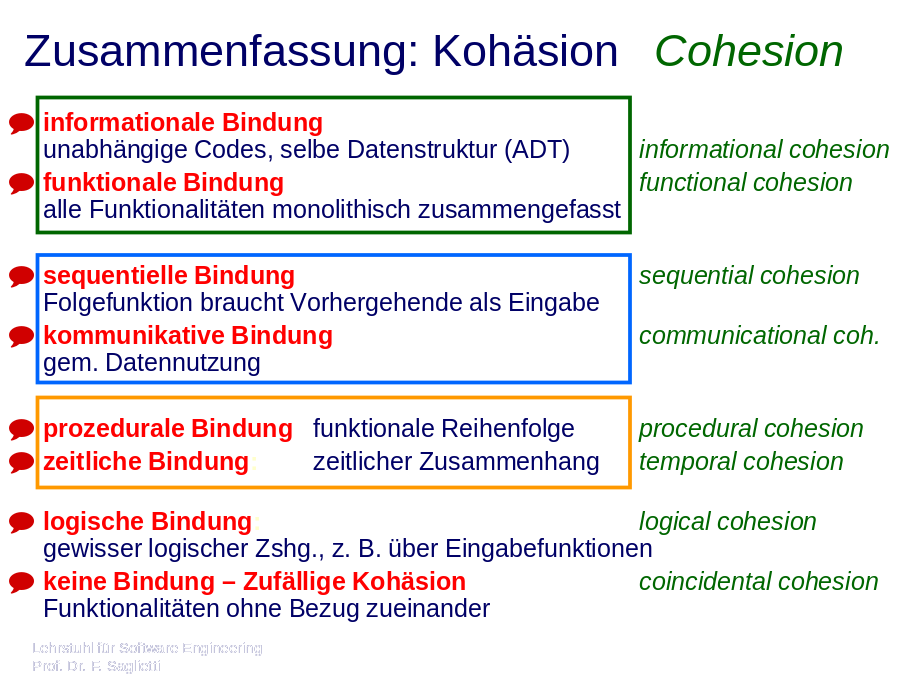
\includegraphics[scale=0.5]{inc/Softwareentwurf/ZusammenfassungKohaesion.png}


\subsubsection{Schlussfolgerung: Grob-Entwurf}

F"ur die Praxis k"onnen aus diesen "Uberlegungen zwei Schlussfolgerungen gezogen werden:
\begin{enumerate}
    \item Wird beim Grob-Entwurf ein Softwaresystem in \textbf{zu wenige} Komponenten zerlegt, so ist im Allgemeinen ein schwacher fuktionaler Zusammenhang innerhalb der Komponente zu erwarten.
    Die wenigen Komponenten werden eher gro"s und un"ubersichtlich sein, was wieder negative Auswirkungen auf die Zuverl"assigkeit und Wartbarkeit hat.
    \item Wird beim Grob-Entwurf ein Softwaresystem in \textbf{zu viele} Komponenten zerlegt, so ist im Allgemeinen ein hoher Grad an Interaktion zwischen den Komponenten zu erwarten.
    Details, die eigentlich innerhalb von Komponenten verborgen bleiben sollten, werden "uber Schnittstellen nach au"sen gegeben, was wiederum negative Auswirkungen auf ide Zuverl"assigkeit und Wartbarkeit hat.
\end{enumerate}



\subsection{Software-Feinentwurf}







